\documentclass{standalone}
\usepackage{pgfplots}

\begin{document}
	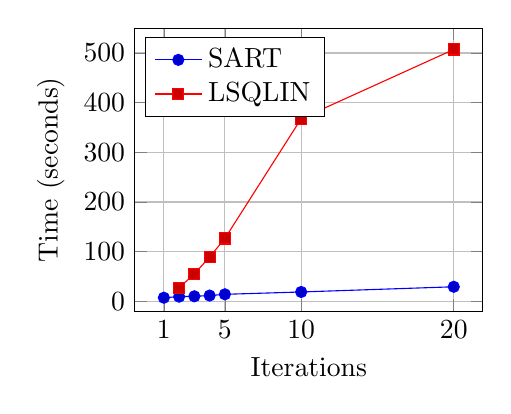
\begin{tikzpicture}
		
		\begin{axis}[	legend pos = north west, 
						legend cell align = left,
						ymin = -20,
						ymax = 550,
						xtick = {1, 5, 10, 20},
						ytick = {0, 100, 200, 300, 400, 500},
						ylabel = {Time (seconds)},
						xlabel = {Iterations},
						ylabel near ticks,
						grid,
						axis on top = false,
						width = 6 cm]
		
			\addplot coordinates {
				(1, 7.0933)
				(2, 9.2096)
				(3, 9.9564)
				(4, 11.4550)
				(5, 13.9412)
				(10, 18.6697)
				(20, 29.1313)
			};
			\addlegendentry{SART};
			
			\addplot coordinates {
				(2, 26.9930)
				(3, 55.2522)
				(4, 89.0784)
				(5, 126.5243)
				(10, 367.7888)
				(20, 507.2163)
			};
			\addlegendentry{LSQLIN};
			
			 
		\end{axis}
		
	\end{tikzpicture}
\end{document}